% Created by tikzDevice version 0.12.3.1 on 2021-04-12 18:47:04
% !TEX encoding = UTF-8 Unicode
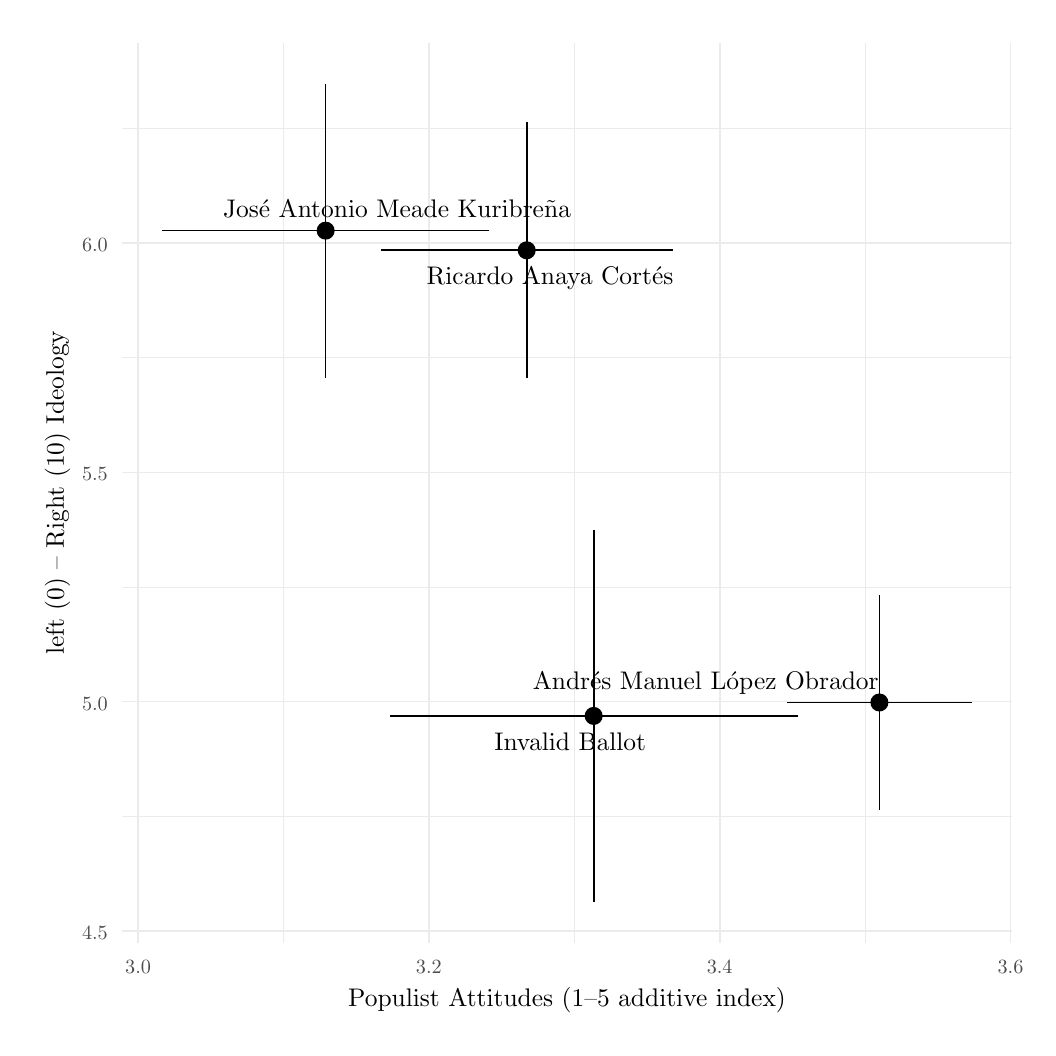
\begin{tikzpicture}[x=1pt,y=1pt]
\definecolor{fillColor}{RGB}{255,255,255}
\path[use as bounding box,fill=fillColor,fill opacity=0.00] (0,0) rectangle (361.35,361.35);
\begin{scope}
\path[clip] ( 33.92, 30.69) rectangle (355.85,355.85);
\definecolor{drawColor}{gray}{0.92}

\path[draw=drawColor,line width= 0.3pt,line join=round] ( 33.92, 76.41) --
	(355.85, 76.41);

\path[draw=drawColor,line width= 0.3pt,line join=round] ( 33.92,159.23) --
	(355.85,159.23);

\path[draw=drawColor,line width= 0.3pt,line join=round] ( 33.92,242.05) --
	(355.85,242.05);

\path[draw=drawColor,line width= 0.3pt,line join=round] ( 33.92,324.87) --
	(355.85,324.87);

\path[draw=drawColor,line width= 0.3pt,line join=round] ( 92.44, 30.69) --
	( 92.44,355.85);

\path[draw=drawColor,line width= 0.3pt,line join=round] (197.52, 30.69) --
	(197.52,355.85);

\path[draw=drawColor,line width= 0.3pt,line join=round] (302.59, 30.69) --
	(302.59,355.85);

\path[draw=drawColor,line width= 0.6pt,line join=round] ( 33.92, 35.00) --
	(355.85, 35.00);

\path[draw=drawColor,line width= 0.6pt,line join=round] ( 33.92,117.82) --
	(355.85,117.82);

\path[draw=drawColor,line width= 0.6pt,line join=round] ( 33.92,200.64) --
	(355.85,200.64);

\path[draw=drawColor,line width= 0.6pt,line join=round] ( 33.92,283.46) --
	(355.85,283.46);

\path[draw=drawColor,line width= 0.6pt,line join=round] ( 39.90, 30.69) --
	( 39.90,355.85);

\path[draw=drawColor,line width= 0.6pt,line join=round] (144.98, 30.69) --
	(144.98,355.85);

\path[draw=drawColor,line width= 0.6pt,line join=round] (250.06, 30.69) --
	(250.06,355.85);

\path[draw=drawColor,line width= 0.6pt,line join=round] (355.13, 30.69) --
	(355.13,355.85);
\definecolor{drawColor}{RGB}{0,0,0}

\path[draw=drawColor,line width= 0.6pt,line join=round] (307.77, 78.61) -- (307.77,156.41);

\path[draw=drawColor,line width= 0.6pt,line join=round] (204.52, 45.47) -- (204.52,179.83);

\path[draw=drawColor,line width= 0.6pt,line join=round] (107.67,234.92) -- (107.67,341.07);

\path[draw=drawColor,line width= 0.6pt,line join=round] (180.32,234.68) -- (180.32,327.12);
\definecolor{fillColor}{RGB}{0,0,0}

\path[draw=drawColor,line width= 0.8pt,line join=round,line cap=round,fill=fillColor] (307.77,117.51) circle (  2.85);

\path[draw=drawColor,line width= 0.8pt,line join=round,line cap=round,fill=fillColor] (204.52,112.65) circle (  2.85);

\path[draw=drawColor,line width= 0.8pt,line join=round,line cap=round,fill=fillColor] (107.67,288.00) circle (  2.85);

\path[draw=drawColor,line width= 0.8pt,line join=round,line cap=round,fill=fillColor] (180.32,280.90) circle (  2.85);

\path[draw=drawColor,line width= 0.6pt,line join=round] (341.22,117.51) --
	(341.22,117.51);

\path[draw=drawColor,line width= 0.6pt,line join=round] (341.22,117.51) --
	(274.33,117.51);

\path[draw=drawColor,line width= 0.6pt,line join=round] (274.33,117.51) --
	(274.33,117.51);

\path[draw=drawColor,line width= 0.6pt,line join=round] (278.29,112.65) --
	(278.29,112.65);

\path[draw=drawColor,line width= 0.6pt,line join=round] (278.29,112.65) --
	(130.75,112.65);

\path[draw=drawColor,line width= 0.6pt,line join=round] (130.75,112.65) --
	(130.75,112.65);

\path[draw=drawColor,line width= 0.6pt,line join=round] (166.79,288.00) --
	(166.79,288.00);

\path[draw=drawColor,line width= 0.6pt,line join=round] (166.79,288.00) --
	( 48.55,288.00);

\path[draw=drawColor,line width= 0.6pt,line join=round] ( 48.55,288.00) --
	( 48.55,288.00);

\path[draw=drawColor,line width= 0.6pt,line join=round] (233.05,280.90) --
	(233.05,280.90);

\path[draw=drawColor,line width= 0.6pt,line join=round] (233.05,280.90) --
	(127.60,280.90);

\path[draw=drawColor,line width= 0.6pt,line join=round] (127.60,280.90) --
	(127.60,280.90);

\node[text=drawColor,anchor=base,inner sep=0pt, outer sep=0pt, scale=  0.92] at (245.01,122.18) {Andrés Manuel López Obrador};

\node[text=drawColor,anchor=base,inner sep=0pt, outer sep=0pt, scale=  0.92] at (196.05,100.29) {Invalid Ballot};

\node[text=drawColor,anchor=base,inner sep=0pt, outer sep=0pt, scale=  0.92] at (133.45,292.68) {José Antonio Meade Kuribreña};

\node[text=drawColor,anchor=base,inner sep=0pt, outer sep=0pt, scale=  0.92] at (188.76,268.59) {Ricardo Anaya Cortés};
\end{scope}
\begin{scope}
\path[clip] (  0.00,  0.00) rectangle (361.35,361.35);
\definecolor{drawColor}{gray}{0.30}

\node[text=drawColor,anchor=base east,inner sep=0pt, outer sep=0pt, scale=  0.73] at ( 28.97, 31.97) {4.5};

\node[text=drawColor,anchor=base east,inner sep=0pt, outer sep=0pt, scale=  0.73] at ( 28.97,114.79) {5.0};

\node[text=drawColor,anchor=base east,inner sep=0pt, outer sep=0pt, scale=  0.73] at ( 28.97,197.61) {5.5};

\node[text=drawColor,anchor=base east,inner sep=0pt, outer sep=0pt, scale=  0.73] at ( 28.97,280.43) {6.0};
\end{scope}
\begin{scope}
\path[clip] (  0.00,  0.00) rectangle (361.35,361.35);
\definecolor{drawColor}{gray}{0.30}

\node[text=drawColor,anchor=base,inner sep=0pt, outer sep=0pt, scale=  0.73] at ( 39.90, 19.68) {3.0};

\node[text=drawColor,anchor=base,inner sep=0pt, outer sep=0pt, scale=  0.73] at (144.98, 19.68) {3.2};

\node[text=drawColor,anchor=base,inner sep=0pt, outer sep=0pt, scale=  0.73] at (250.06, 19.68) {3.4};

\node[text=drawColor,anchor=base,inner sep=0pt, outer sep=0pt, scale=  0.73] at (355.13, 19.68) {3.6};
\end{scope}
\begin{scope}
\path[clip] (  0.00,  0.00) rectangle (361.35,361.35);
\definecolor{drawColor}{RGB}{0,0,0}

\node[text=drawColor,anchor=base,inner sep=0pt, outer sep=0pt, scale=  0.92] at (194.89,  7.64) {Populist Attitudes (1--5 additive index)};
\end{scope}
\begin{scope}
\path[clip] (  0.00,  0.00) rectangle (361.35,361.35);
\definecolor{drawColor}{RGB}{0,0,0}

\node[text=drawColor,rotate= 90.00,anchor=base,inner sep=0pt, outer sep=0pt, scale=  0.92] at ( 13.08,193.27) {left (0) -- Right (10) Ideology};
\end{scope}
\end{tikzpicture}
